\documentclass[12pt,a4paper]{article}
\usepackage[utf8]{inputenc}
\usepackage[T1]{fontenc}
\usepackage{lmodern}          % vektorski (Type 1) fontovi umesto bitmap-a
\usepackage{microtype}        % micro-typografija: kerning, word spacing
\usepackage[serbian]{babel}
\usepackage{amsmath, amssymb}
\usepackage{graphicx}
\usepackage{booktabs}
\usepackage{array}
\usepackage{float}
\usepackage{caption}
\usepackage{geometry}
\usepackage{hyperref}
\geometry{margin=2.5cm}
\graphicspath{{./}{plots/}}   % logo je u src/homework_3/, grafici u plots/

\begin{document}

% ── Naslovna strana ───────────────────────────────────────────────────────────
\begin{titlepage}
  \centering
  \vspace*{1.5cm}
  
\includegraphics[width=0.32\textwidth]{etf_logo.png}\\[1.8cm]
  {\large Univerzitet u Beogradu}\\[0.3em]
  {\large Elektrotehnički fakultet}\\[2.5cm]
  {\LARGE\textbf{Treći domaći zadatak}}\\[0.8em]
  {\Large Učenje podsticanjem}\\[0.6em]
  {\large Predmet: Veštačka inteligencija (13E053VI)}\\[3.5cm]
  {\large Mihajlo Stevanović}\\[0.3em]
  {\large 2022/0315}\\[2cm]
  {\large Beograd, \the\year}
\end{titlepage}

% =============================================================================
\section{Opis okruženja i simulator}
% =============================================================================

Okruženje je mreža dimenzija $2 \times 5$ sa stanjima označenim kao $A_1,\ldots,A_5$
(gornji red) i $B_1,\ldots,B_5$ (donji red), prikazana u tabeli~\ref{tab:grid}.
Stanja $B_1$, $B_3$ i $B_5$ su terminalna. Agent dobija nagradu $-1$ pri prelasku
u $B_1$ ili $B_5$, nagradu $+1$ pri prelasku u $B_3$, i nagradu $-0{,}04$
(tzv.\ ,,living cost'') u svakom koraku koji ne završava epizodu.
Faktor diskontovanja je $\gamma = 0{,}9$ (ako nije navedeno drugačije).
Na početku svake epizode agent uniformno bira jedno od 7 neterminalnih stanja.

\begin{table}[H]
  \centering
  \caption{Struktura okruženja $2\times5$.}
  \begin{tabular}{c|ccccc}
    \toprule
         & kol 1 & kol 2 & kol 3 & kol 4 & kol 5 \\
    \midrule
    red A & $A_1$ & $A_2$ & $A_3$ & $A_4$ & $A_5$ \\
    red B & $B_1\;(-1)$ & $B_2$ & $B_3\;(+1)$ & $B_4$ & $B_5\;(-1)$ \\
    \bottomrule
  \end{tabular}
  \label{tab:grid}
\end{table}

\subsection{Model prelaza}

Agent raspolaže sa četiri akcije: \emph{gore}, \emph{dole}, \emph{levo},
\emph{desno}. Okruženje je stohastično:
\[
P(s' \mid s, a) =
\begin{cases}
  0{,}6 & \text{ako } s' = \mathrm{move}(s,a) \text{ (nameravani smer)}\\
  0{,}1 & \text{za svaki od preostala 3 smera}\\
  0{,}1 & \text{,,ostani u mestu'' (nema pomeraja)}
\end{cases}
\]
Pokušaj izlaska iz mreže ne menja stanje agenta (udarac u zid).
Model zadovoljava Markovljevu osobinu: naredno stanje $s'$ zavisi samo od tekućeg
stanja $s$ i izabrane akcije $a$.

\paragraph{Verifikacija.}
Za stanje $A_1$ i akciju \emph{desno}: desno$\to A_2$ (0{,}6),
gore$\to$zid$\to A_1$ (0{,}1), levo$\to$zid$\to A_1$ (0{,}1),
ostani$\to A_1$ (0{,}1), dole$\to B_1$ (0{,}1):
\[
P(A_2 \mid A_1, \text{desno}) = 0{,}6,\quad
P(A_1 \mid A_1, \text{desno}) = 0{,}3,\quad
P(B_1 \mid A_1, \text{desno}) = 0{,}1.
\]
Ovi rezultati se poklapaju sa primerom iz teksta zadatka.

\subsection{Simulator}

Implementirani simulator drži interno stanje $s$. Pozivom \texttt{step}$(a)$
sempluje naredno stanje $s' \sim P(\cdot \mid s, a)$, izračunava nagradu
$r = R(s')$ i vraća trojku $(r,\, s',\, \text{done})$.
Metoda \texttt{reset()} uniformno bira jedno od 7 neterminalnih stanja.
Metoda \texttt{model}$(s,a)$ izlaže $P(\cdot \mid s, a)$ kao rečnik;
sme je koristiti \emph{jedino} iteracija Q-vrednosti.


% =============================================================================
\section{Iteracija Q-vrednosti (etalon)}
% =============================================================================

\subsection{Algoritam}

Q-vrednost para $(s, a)$ predstavlja očekivani diskontovani prinos pri primeni
akcije $a$ u stanju $s$ uz naknadno praćenje optimalne politike:
\[
Q^*(s, a) = \sum_{s'} P(s' \mid s, a)
  \Bigl[R(s') + \gamma \max_{a'} Q^*(s', a')\Bigr].
\]

Iterativna procedura polazi od $Q_0(s,a) = 0$ za sve $(s,a)$ i primenjuje
sinhrone Belmanove projekcije:
\[
Q_{t+1}(s, a) = \sum_{s'} P(s' \mid s, a)
  \Bigl[R(s') + \gamma \max_{a'} Q_t(s', a')\Bigr],
  \quad \forall (s,a) \in \mathcal{S}_{\mathrm{NT}} \times \mathcal{A}.
\]
Za terminalna stanja važi $\max_{a'} Q(s', a') = 0$.
Algoritam konvergira ka $Q^*$ jer je Belmanov operator kontrakcija sa konstantom
$\gamma$:
\[
\|Q_{t+1} - Q^*\|_\infty \;\leq\; \gamma \cdot \|Q_t - Q^*\|_\infty
\;\longrightarrow\; 0.
\]
Iz $Q^*$ direktno slede optimalna vrednosna funkcija i politika:
\[
V^*(s) = \max_a Q^*(s,a), \qquad
\pi^*(s) = \arg\max_a Q^*(s,a).
\]

\subsection{Rezultati}

Algoritam konvergira za \textbf{53 iteracije} pri $\gamma = 0{,}9$
(tolerancija $\|\delta Q\|_\infty < 10^{-12}$).

\begin{figure}[H]
  \centering
  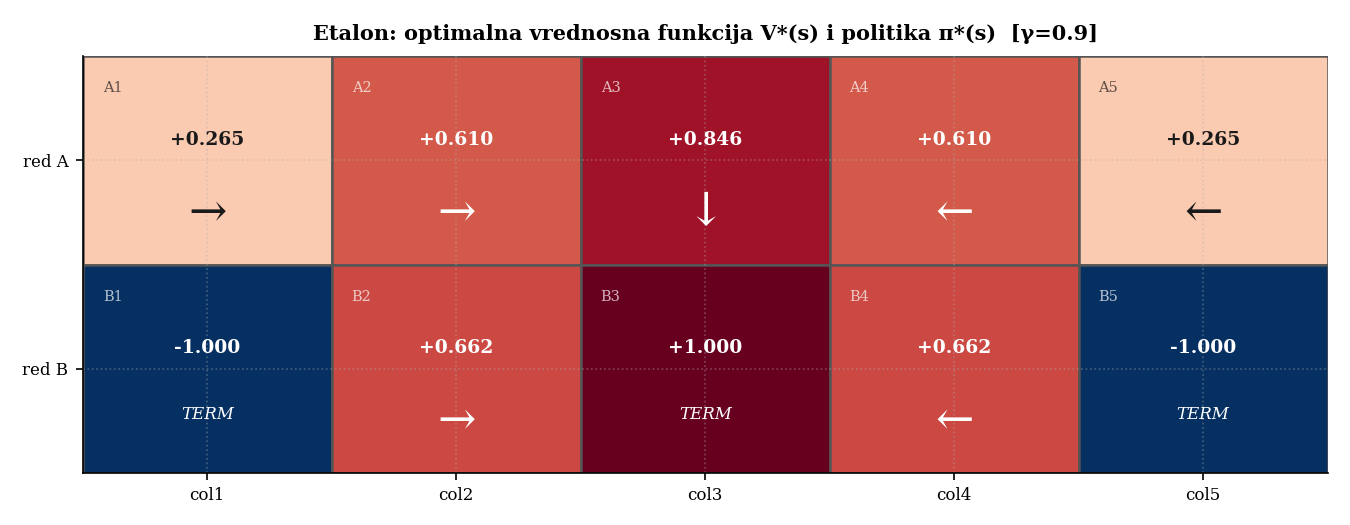
\includegraphics[width=0.85\textwidth]{G1_Vstar_pistar.png}
  \caption{Optimalne vrednosti $V^*(s)$ (heatmap: crvena = $-1$, bela = $0$, plava = $+1$)
           i optimalna politika $\pi^*(s)$ (strelice), $\gamma = 0{,}9$.
           Vrednosti rastu ka centrima i simetrične su oko kolone 3.
           Sva stanja reda $A$ usmeravaju agenta ka sredini ($A_3$),
           odakle on ide dole direktno u terminal $B_3$ ($+1$).
           Stanja $B_2$ i $B_4$ idu direktno desno, odnosno levo, ka $B_3$.}
  \label{fig:g1}
\end{figure}

\begin{table}[H]
  \centering
  \caption{Optimalne V-vrednosti $V^*(s)$ za $\gamma = 0{,}9$.}
  \begin{tabular}{lcccccc}
    \toprule
    Stanje  & $A_1$ & $A_2$ & $A_3$ & $A_4$ & $A_5$ & $B_2 = B_4$ \\
    \midrule
    $V^*(s)$ & $+0{,}265$ & $+0{,}610$ & $+0{,}846$ & $+0{,}610$ & $+0{,}265$
             & $+0{,}662$ \\
    $\pi^*(s)$ & desno & desno & dole & levo & levo & desno / levo \\
    \bottomrule
  \end{tabular}
  \label{tab:vstar}
\end{table}

Vrednost $V^*(A_3) = 0{,}846$ ne dostiže $+1$ zbog živog troška $(-0{,}04)$
i stohastičnosti prelaza.
Za $\gamma = 0{,}999$ algoritam konvergira za \textbf{66 iteracija}, jer je stopa
konvergencije $\gamma^t$ sporija kada je $\gamma$ bliže 1.

\begin{figure}[H]
  \centering
  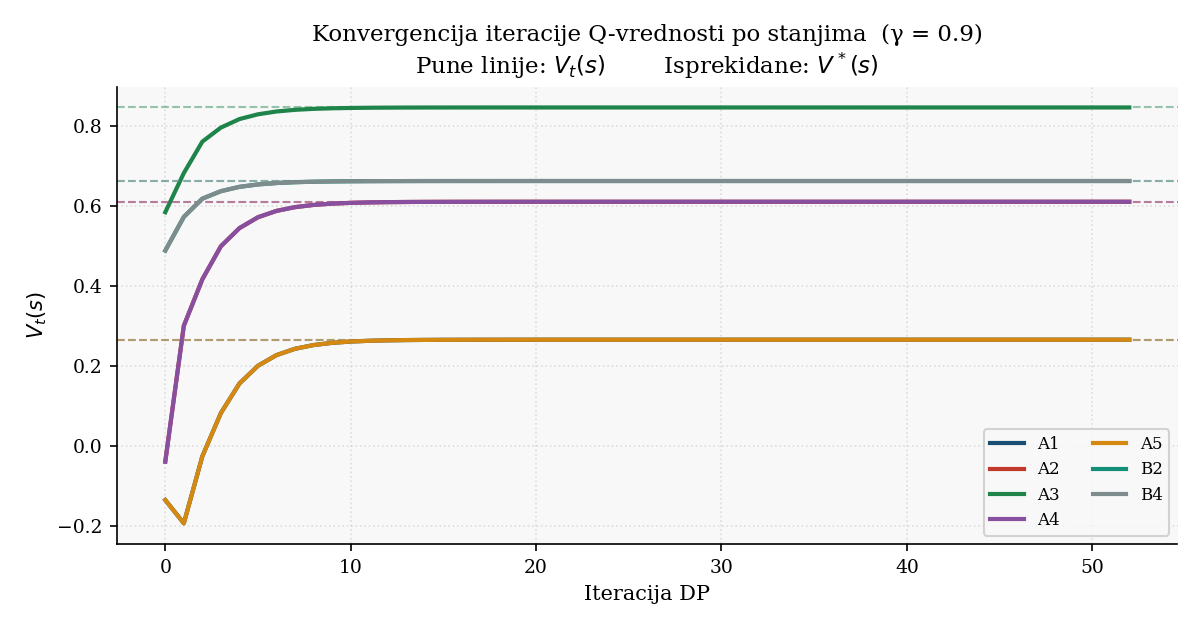
\includegraphics[width=0.82\textwidth]{G2_QVI_konvergencija.png}
  \caption{Konvergencija iteracije Q-vrednosti ($\gamma = 0{,}9$):
           $V_t(s) = \max_a Q_t(s,a)$ u zavisnosti od iteracije $t$.
           Pune linije prikazuju $V_t(s)$; isprekidane horizontale označavaju $V^*(s)$.
           Konvergencija je geometrijska sa stopom $\gamma^t$: vrednosti se stabilizuju
           unutar prvih 20--25 iteracija.
           Stanja bliža terminalu $B_3$ (npr.\ $A_3$, $B_2$, $B_4$) konvergiraju
           brže jer im lanci zavisnosti od terminalne nagrade imaju manje karika.}
  \label{fig:g2}
\end{figure}


% =============================================================================
\section{Q-učenje}
% =============================================================================

\subsection{Algoritam}

Q-učenje je TD (,,temporal difference'') algoritam \emph{bez modela} (model-free).
Uči Q-vrednosti direktno iz osmotrenih četvorki $(s, a, r, s')$, bez pristupa
modelu prelaza $P(s' \mid s, a)$.
Nakon svakog prelaza vrši se ažuriranje:
\[
Q(s, a) \;\leftarrow\; Q(s, a) + \alpha
  \underbrace{\bigl[r + \gamma \max_{a'} Q(s', a') - Q(s, a)\bigr]}_{\text{TD greška }
  \delta},
\]
gde se za terminalna stanja $s'$ uzima $\max_{a'} Q(s', a') = 0$.
Algoritam je \emph{off-policy}: cilj koristi $\max_{a'}$ bez obzira na izabranu
akciju u $s'$, pa $\varepsilon$-gramziva politika utiče samo na pokrivenost prostora,
a ne na vrednost ka kojoj konvergiramo.

\paragraph{$\varepsilon$-gramzivo istraživanje.}
\[
a \;=\; \begin{cases}
  \text{slučajna akcija}   & \text{s verovatnoćom } \varepsilon \\
  \arg\max_a Q(s, a)       & \text{s verovatnoćom } 1 - \varepsilon
\end{cases}
\]
Izjednačenja u $\arg\max$ razrešavaju se nasumično kako bi se izbegla inicijalna
pristrasnost (na startu su svi $Q = 0$, pa bi deterministički izbor uvek favorizovao
istu akciju).

\paragraph{Uslovi konvergencije (Robbins--Monro).}
Neophodan i dovoljan uslov za konvergenciju Q-učenja ka $Q^*$ je:
\[
\sum_{e=1}^{\infty} \alpha_e = \infty \qquad \text{i} \qquad
\sum_{e=1}^{\infty} \alpha_e^2 < \infty.
\]
Razmatrane su dve strategije stope učenja:
\begin{itemize}
  \item \textbf{Promenljiva:} $\displaystyle\alpha_e = \frac{\ln(e+1)}{e+1}$:
    zadovoljava oba uslova, Q konvergira u tačku ka $Q^*$.
  \item \textbf{Konstantna:} $\alpha_e = c$: narušava drugi uslov
    ($\sum c^2 = \infty$), Q ,,treperi'' oko $Q^*$ sa rezidualom $\propto c$.
\end{itemize}

\subsection{Izbor parametra $\varepsilon$}

Primenjivali smo Q-učenje sa promenljivom stopom $\alpha_e = \ln(e+1)/(e+1)$
za vrednosti $\varepsilon \in \{0;\; 0{,}05;\; 0{,}1;\; 0{,}2;\; 0{,}3\}$
kroz 20 nezavisnih izvođenja i 10\,000 epizoda po izvođenju.
Rezultati su prikazani na slici~\ref{fig:g5}.

\begin{figure}[H]
  \centering
  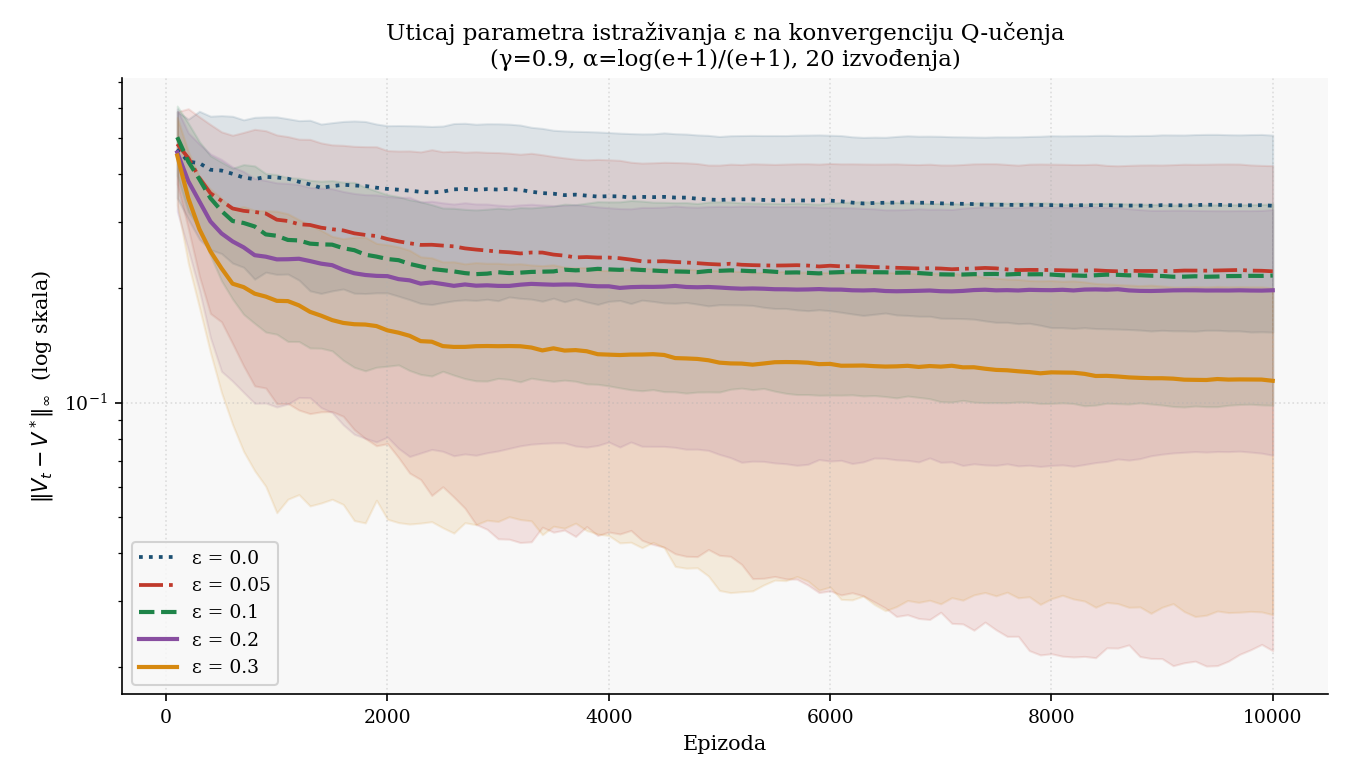
\includegraphics[width=0.82\textwidth]{G5_QL_epsilon_poredjenje.png}
  \caption{Uticaj $\varepsilon$ na brzinu konvergencije Q-učenja:
           $\|V_t - V^*\|_\infty$ u zavisnosti od broja epizoda
           (srednja vrednost $\pm$ std za 20 nezavisnih izvođenja,
           $\gamma = 0{,}9$, $\alpha_e = \ln(e+1)/(e+1)$).
           $\varepsilon = 0$ zaostaje jer agent nikada ne istražuje alternativne akcije.
           Vrednosti $\varepsilon \in \{0{,}1;\; 0{,}2\}$ postižu najbrže opadanje greške.
           Preveliko $\varepsilon = 0{,}3$ troši korake na nasumične akcije i usporava
           konvergenciju u kasnijim fazama.}
  \label{fig:g5}
\end{figure}

Zbog uniformne raspodele početnih stanja, agent prirodno posećuje sva neterminalna
stanja bez agresivnog istraživanja; $\varepsilon$ je prevashodno potreban
da bi agent isprobavao \emph{alternativne akcije} u svakom stanju.
Odabrana vrednost je $\varepsilon^* = 0{,}1$.

\subsection{Konvergencija i poređenje stopa učenja}

Slika~\ref{fig:g3} prikazuje kako se $V_t(s)$ menja tokom učenja i konvergira
ka etalonu $V^*(s)$ za svako od 7 stanja.

\begin{figure}[H]
  \centering
  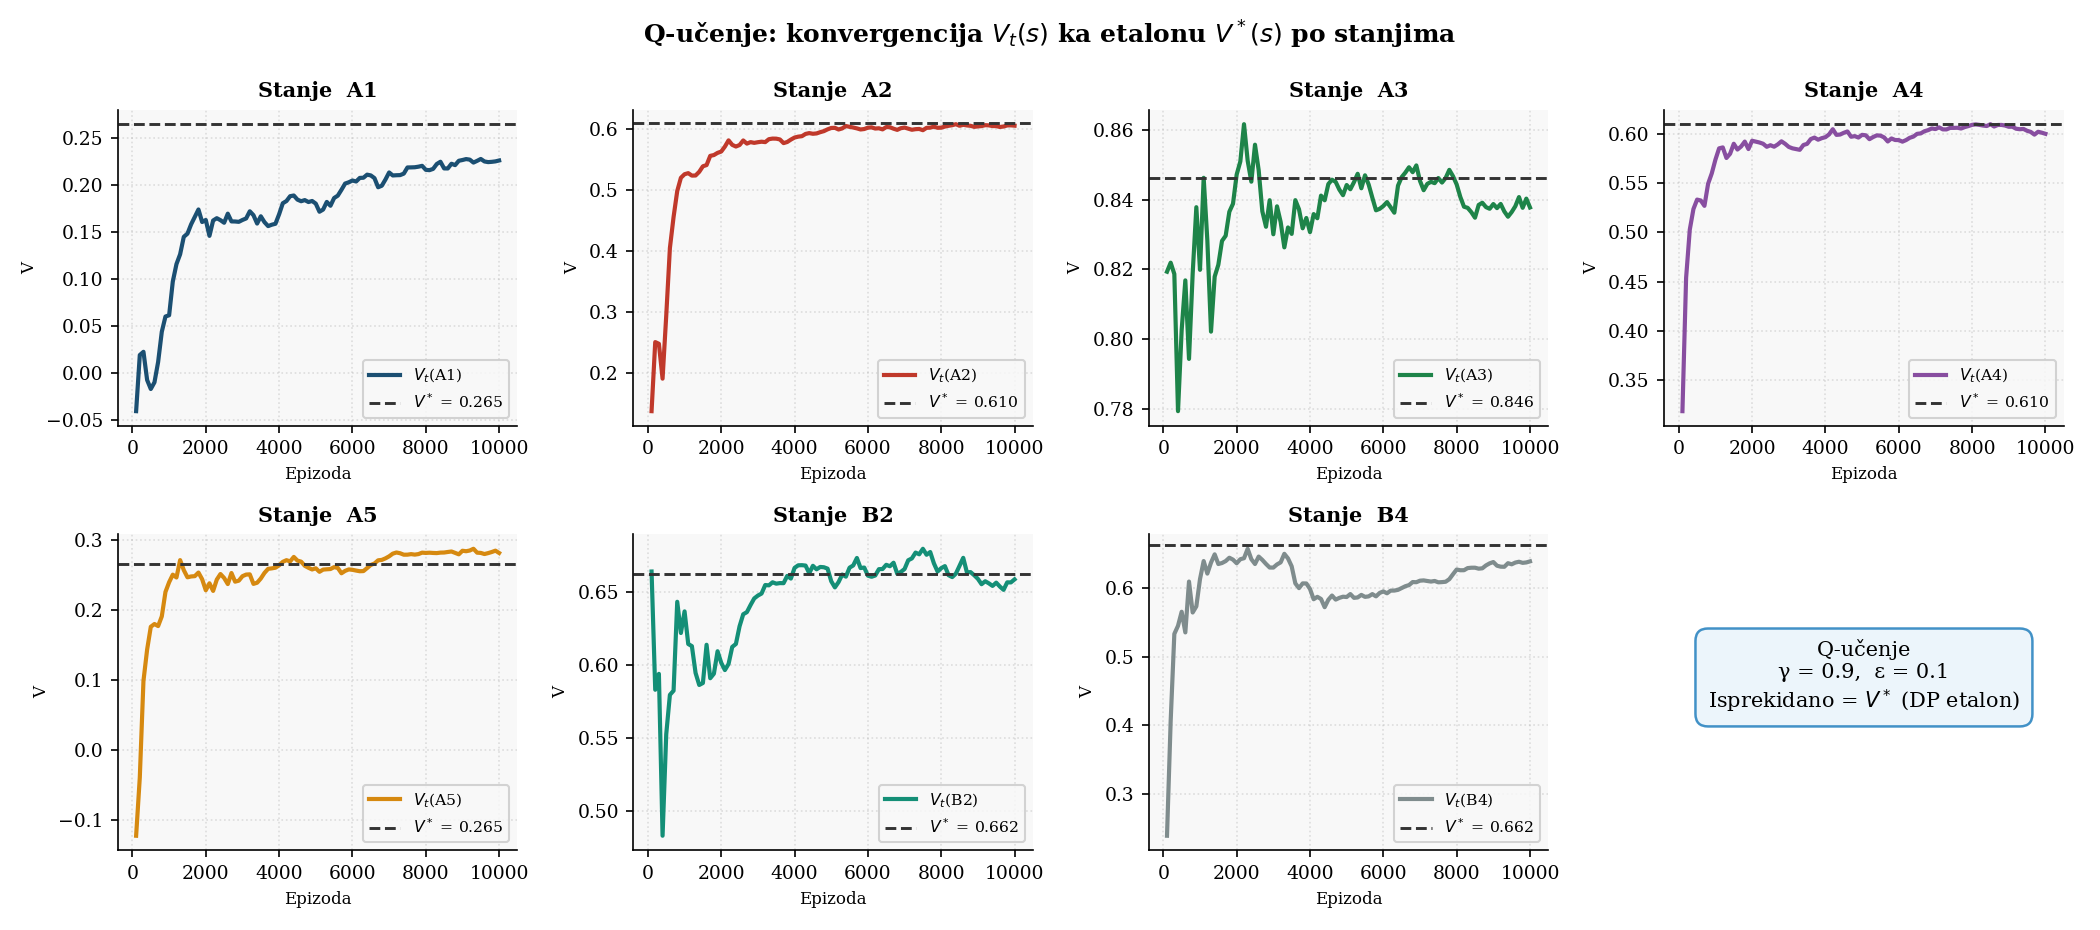
\includegraphics[width=\textwidth]{G3_QL_Vt_po_stanjima.png}
  \caption{Q-učenje ($\gamma = 0{,}9$, $\varepsilon = 0{,}1$,
           $\alpha_e = \ln(e+1)/(e+1)$, 10\,000 epizoda):
           $V_t(s) = \max_a Q_t(s,a)$ u zavisnosti od broja epizoda.
           Isprekidana horizontalna linija označava $V^*(s)$ iz DP etalona.
           Svaka puna linija se stabilizuje oko svoje isprekidane;
           razlika između postignutih $V_t$ i etalona kretala se od $0{,}003$ (stanje $B_2$)
           do $0{,}039$ (stanje $A_1$) — ugaono stanje koje agent najređe posećuje
           jer uniformni restart ne favorizuje ivice mreže.}
  \label{fig:g3}
\end{figure}

\begin{figure}[H]
  \centering
  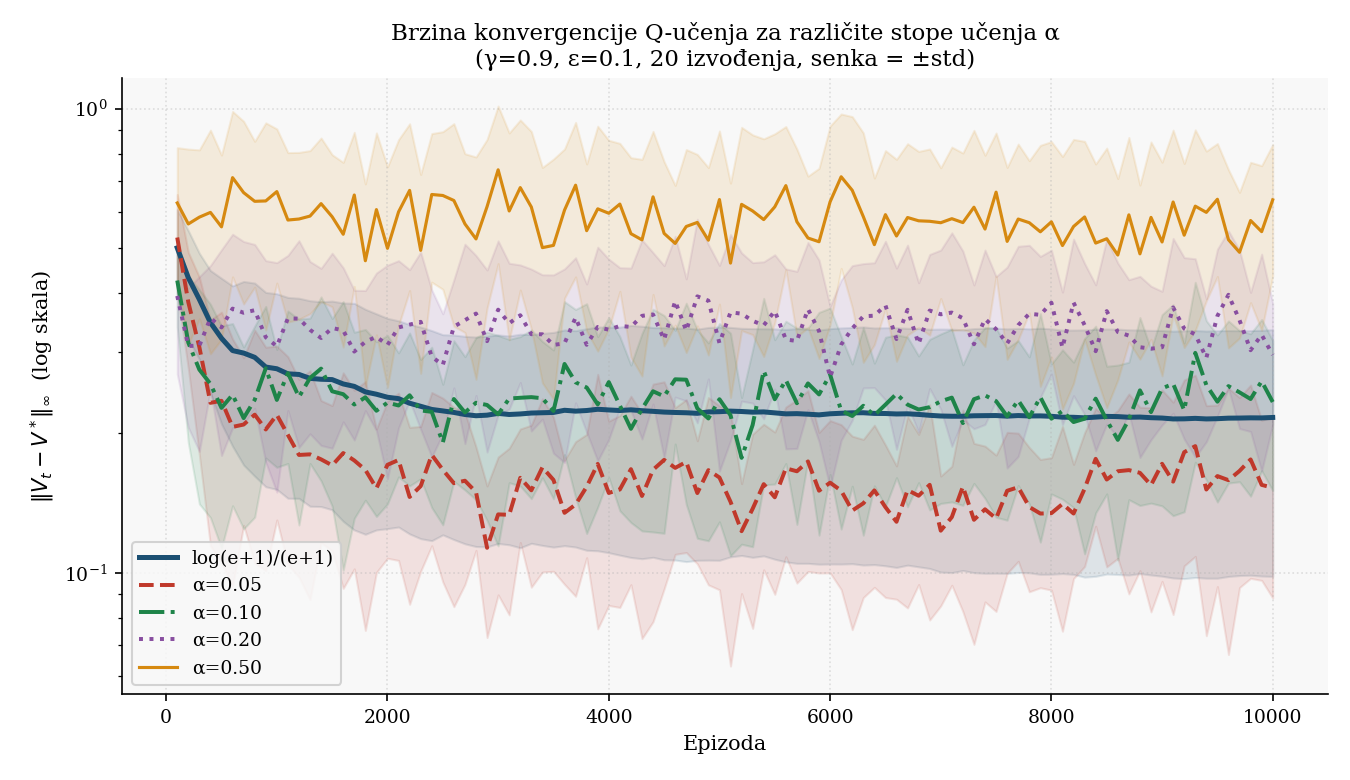
\includegraphics[width=0.82\textwidth]{G4_QL_alpha_poredjenje.png}
  \caption{Poređenje stopa učenja za Q-učenje ($\gamma = 0{,}9$, $\varepsilon = 0{,}1$,
           20 nezavisnih izvođenja): $\|V_t - V^*\|_\infty$ u zavisnosti od broja epizoda.
           Senke prikazuju $\pm$ standardna devijacija.
           Promenljiva stopa $\ln(e+1)/(e+1)$ dostiže najniži asimptotski nivo greške
           jer zadovoljava Robbins--Monro uslove.
           Konstantne stope konvergiraju brže u ranoj fazi, ali se stabilizuju na nenultom
           platou čija visina raste sa $\alpha$ (rezidualna varijansa $\propto \alpha$).
           Preveliko $\alpha = 0{,}50$ izaziva nestabilnost ažuriranja.}
  \label{fig:g4}
\end{figure}

U ovom eksperimentu promenljiva stopa završava sa najnižom greškom na svim stanjima,
dok konstantne stope stabilno platoiraju iznad nje na visini $\propto \alpha$.
Za primene gde je važna finalna preciznost preporučuje se opadajuća stopa;
za brz inicijalni napredak može se krenuti sa većim konstantnim $\alpha$,
pa ga postepeno gasiti kako varijansa pada (tzv.\ ,,annealing'').

\subsection{Uticaj faktora diskontovanja $\gamma$}

\begin{figure}[H]
  \centering
  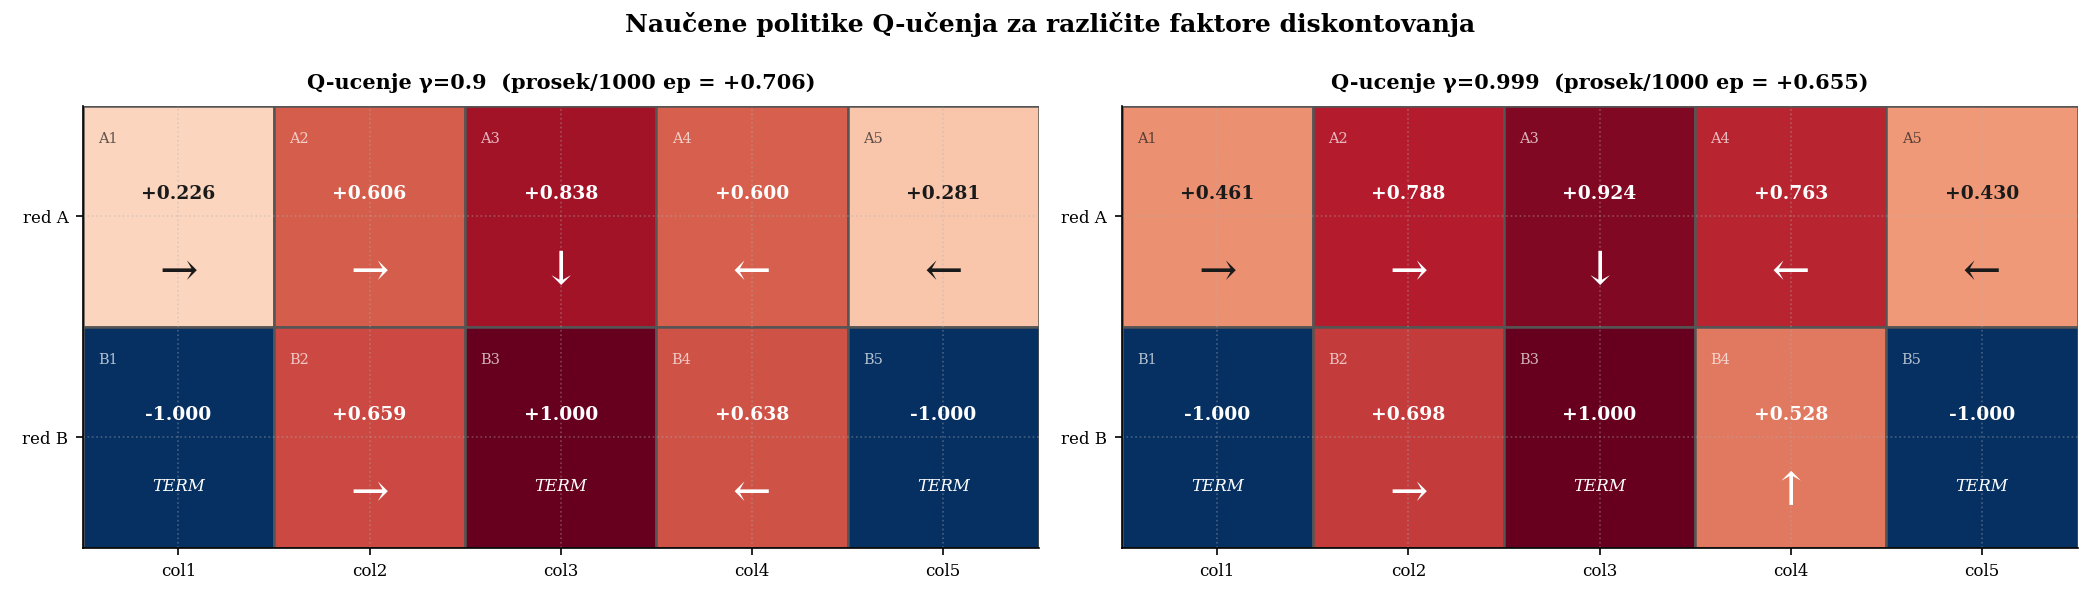
\includegraphics[width=\textwidth]{G6_QL_gamma_poredjenje.png}
  \caption{Naučene politike Q-učenja za $\gamma = 0{,}9$ (levo) i $\gamma = 0{,}999$
           (desno) posle 10\,000 epizoda.
           V-vrednosti su znatno veće za $\gamma = 0{,}999$ jer agent gotovo jednako
           vrednuje buduće i trenutne nagrade.
           Politike su identične u šest od sedam stanja; stanje $B_4$ pri $\gamma = 0{,}999$
           može pokazati drugačiju akciju, što ukazuje da 10\,000 epizoda nije dovoljno
           za potpunu konvergenciju pri velikom $\gamma$ (konvergencija DP je geometrijska
           sa stopom $\gamma^t$, sporija za veće $\gamma$).}
  \label{fig:g6}
\end{figure}

\begin{table}[H]
  \centering
  \caption{Prosečna ukupna nagrada greedy politike Q-učenja za različite $\gamma$.}
  \begin{tabular}{lcc}
    \toprule
    & $\gamma = 0{,}9$ & $\gamma = 0{,}999$ \\
    \midrule
    Prosek / 10 epizoda   & $+0{,}668$ & $+0{,}440$ \\
    Prosek / 1\,000 epizoda & $+0{,}706$ & $+0{,}655$ \\
    \bottomrule
  \end{tabular}
  \label{tab:gamma}
\end{table}

\textbf{Tumačenje.}
Agent sa $\gamma = 0{,}999$ je ,,dalekovidiji'' i praktično jednako vrednuje
nagrade bez obzira na vremensku udaljenost.
To ga motiviše da preferira putanje koje minimizuju ukupni living cost,
čak po cenu duljeg puta, jer je spremniji da plati više koraka od $-0{,}04$
da bi sigurno izbegao terminale $-1$.
Agent sa $\gamma = 0{,}9$ jače diskontuje udaljene nagrade i prihvata veći rizik
od terminala $-1$ u zamenu za kraću putanju.

Sa aspekta konvergencije: DP konvergira za 53 iteracije pri $\gamma = 0{,}9$,
ali za 66 iteracija pri $\gamma = 0{,}999$, jer je stopa $\gamma^t$ sporija.
Analogno, Q-učenje zahteva više epizoda za isti kvalitet aproksimacije pri $\gamma = 0{,}999$,
što se ogleda u nižoj prosečnoj nagradi pri jednakom broju epizoda (tabela~\ref{tab:gamma}).


% =============================================================================
\section{REINFORCE}
% =============================================================================

\subsection{Parametrizacija politike}

REINFORCE je algoritam gradijenta politike (policy gradient) koji direktno
optimizuje parametre $\boldsymbol\theta$ politike $\pi_\theta$, bez eksplicitnog
učenja vrednosne funkcije.
Pošto su akcije diskretne ($|\mathcal{A}| = 4$), prirodna i standardna parametrizacija
je \textbf{softmaks po parovima (stanje, akcija)}:
\[
\pi_\theta(a \mid s) = \frac{\exp(\theta_{s,a})}{\displaystyle\sum_{a'}
  \exp(\theta_{s,a'})},
\]
sa po jednim realnim parametrom $\theta_{s,a}$ za svako neterminalno stanje $s$
i svaku akciju $a$.
Ukupno se uči $7 \times 4 = \mathbf{28}$ parametara.
Inicijalizacija $\theta_{s,a} = 0$ daje uniformnu politiku
$\pi(a \mid s) = 1/4$ za sve akcije (neutralan, nepristrasan početak).

Nasuprot Gausovoj politici (koja je standardna za \emph{kontinualne} akcije),
softmaks direktno modeluje raspodelu verovatnoća nad diskretnim skupom akcija.
Svaki parametar $\theta_{s,a}$ se interpretira kao ,,logit'' (relativna preferencija
akcije $a$ u stanju $s$), što ga čini pogodnim za grafičko praćenje i intuitivno tumačenje.

\subsection{Algoritam}

Cilj je maksimizovati očekivani prinos $J(\theta) = \mathbb{E}_{\pi_\theta}[G_0]$.
Po \emph{teoremi o gradijentu politike}:
\[
\nabla_\theta J(\theta) = \mathbb{E}_{\pi_\theta}\!\Bigl[
  \sum_\tau v_\tau \cdot \nabla_\theta \ln \pi_\theta(a_\tau \mid s_\tau)
\Bigr],
\]
gde je $v_\tau$ \textbf{return-to-go} (povraćaj-do-kraja):
\[
v_\tau = r_\tau + \gamma r_{\tau+1} + \gamma^2 r_{\tau+2} + \cdots
       = r_\tau + \gamma v_{\tau+1}, \qquad v_T = 0.
\]
Korišćenjem return-to-go umesto pune epizodne sume $G_0$ eliminišemo uticaj
prošlih nagrada (koje ne zavise od akcije u koraku $\tau$), čime se smanjuje
varijansa gradijenta bez uvođenja pristrasnosti.

Za softmaks politiku, gradijent log-politike ima zatvorenu formu (skor funkcija):
\[
\frac{\partial}{\partial \theta_{s,a'}} \ln \pi_\theta(a \mid s)
= \mathbf{1}[a' = a] - \pi_\theta(a' \mid s).
\]

Ažuriranje parametara za svaki korak $\tau$ epizode:
\[
\theta_{s_\tau, a'} \;\leftarrow\; \theta_{s_\tau, a'}
  + \alpha \cdot v_\tau \cdot \bigl(\mathbf{1}[a' = a_\tau]
    - \pi_\theta(a' \mid s_\tau)\bigr), \quad \forall a' \in \mathcal{A}.
\]
Za izabranu akciju ($a' = a_\tau$) gradijent je pozitivan ($1 - \pi > 0$),
što znači da njena verovatnoća raste.
Za sve ostale akcije gradijent je negativan, te njihova verovatnoća opada.
Efekat je proporcionalan $v_\tau$: dobre epizode ($v_\tau > 0$) povećavaju
verovatnoću izabranih akcija, loše ($v_\tau < 0$) je smanjuju.

Procena gradijenta po jednoj trajektoriji je nepristrasna, ali visoke varijanse:
bez bootstrappinga, jedan prinos $G_0$ je tek jedan Monte Carlo uzorak očekivanja
$J(\theta)$. Posledica je vidljiva direktno u G7 — sirova kriva osciluje između
$\approx -1{,}5$ i $+1{,}0$ kroz sve epizode, a tek klizni prosek otkriva trend.

\subsection{Kriva učenja}

\begin{figure}[H]
  \centering
  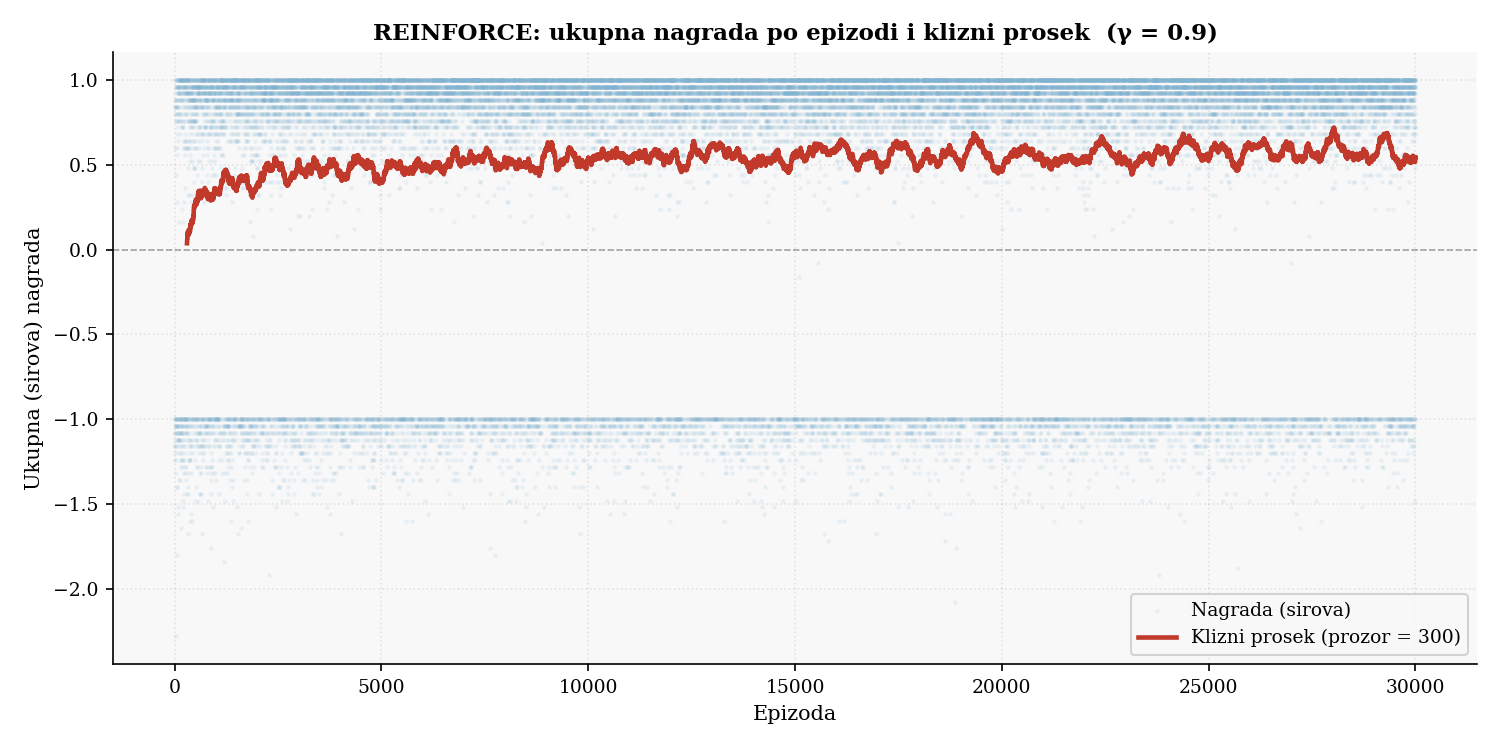
\includegraphics[width=0.90\textwidth]{G7_RF_kriva_ucenja.png}
  \caption{REINFORCE ($\gamma = 0{,}9$, $\alpha_e = \ln(e+1)/(e+1)$, 30\,000 epizoda):
           sirova ukupna nagrada po epizodi (svetloplavi tačkasti prikaz)
           i klizni prosek s prozorom 300 epizoda (crvena linija).
           Kriva pokazuje jasan uzlazni trend: prosek prvih 1\,000 epizoda je $+0{,}24$,
           a poslednjih 1\,000 epizoda je $+0{,}57$.
           Visoka varijansa je inherentna karakteristika Monte Carlo gradijenta:
           bez bootstrappinga, ukupan prinos jedne epizode je bučna procena
           očekivane vrednosti gradijenta.}
  \label{fig:g7}
\end{figure}

\subsection{Evolucija parametara i verovatnoća politike}

\begin{figure}[H]
  \centering
  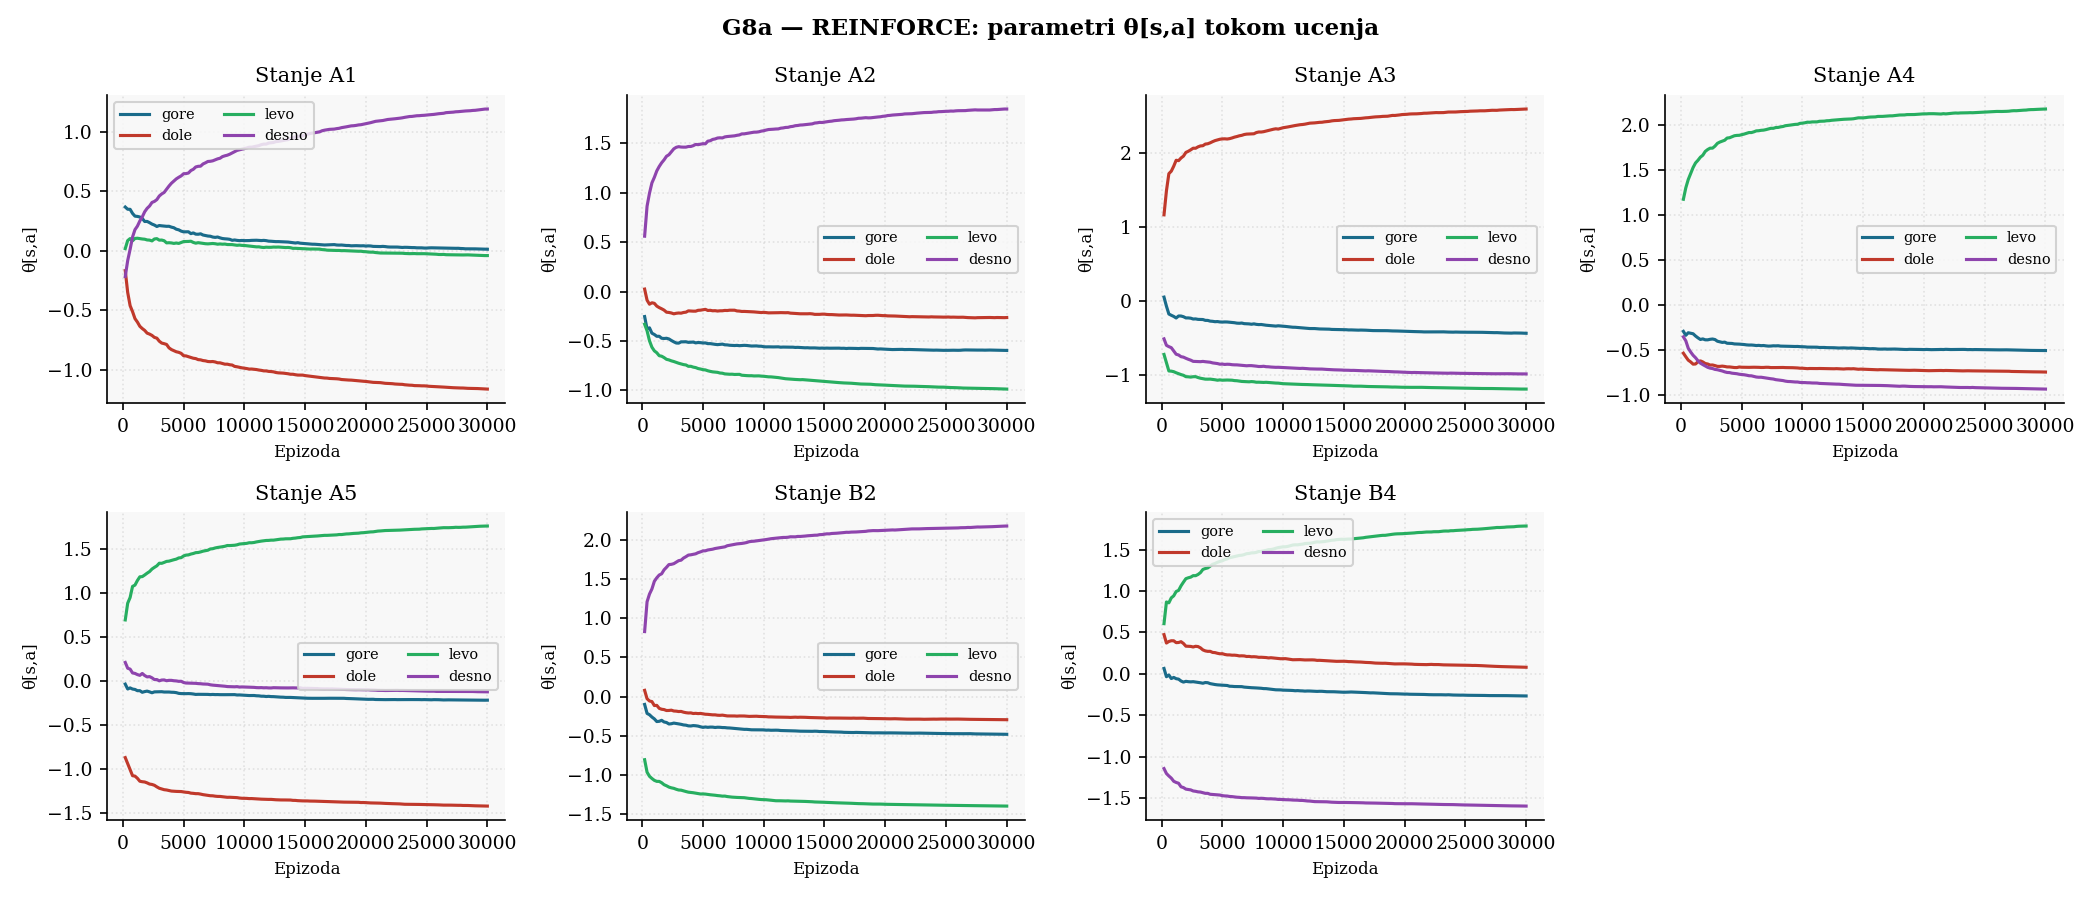
\includegraphics[width=\textwidth]{G8a_RF_theta.png}
  \caption{Vrednosti parametara $\theta_{s,a}$ tokom učenja za svih 7 neterminalnih
           stanja (po jedan podgrafik po stanju, 4 krive po akciji).
           U svakom stanju parametar optimalne akcije monotono raste, dok ostali opadaju.
           Najizraženiji signal je u stanju $A_3$: parametar akcije \emph{dole} (ka $B_3$)
           dostiže vrednosti višestruko veće od ostalih, pošto je
           $A_3 \to B_3$ direktan jednokoračni put do terminalne nagrade $+1$.
           Parametri stanja $A_1$ i $A_5$ rastu sporije jer su ugaona, retko posećena stanja.}
  \label{fig:g8a}
\end{figure}

\begin{figure}[H]
  \centering
  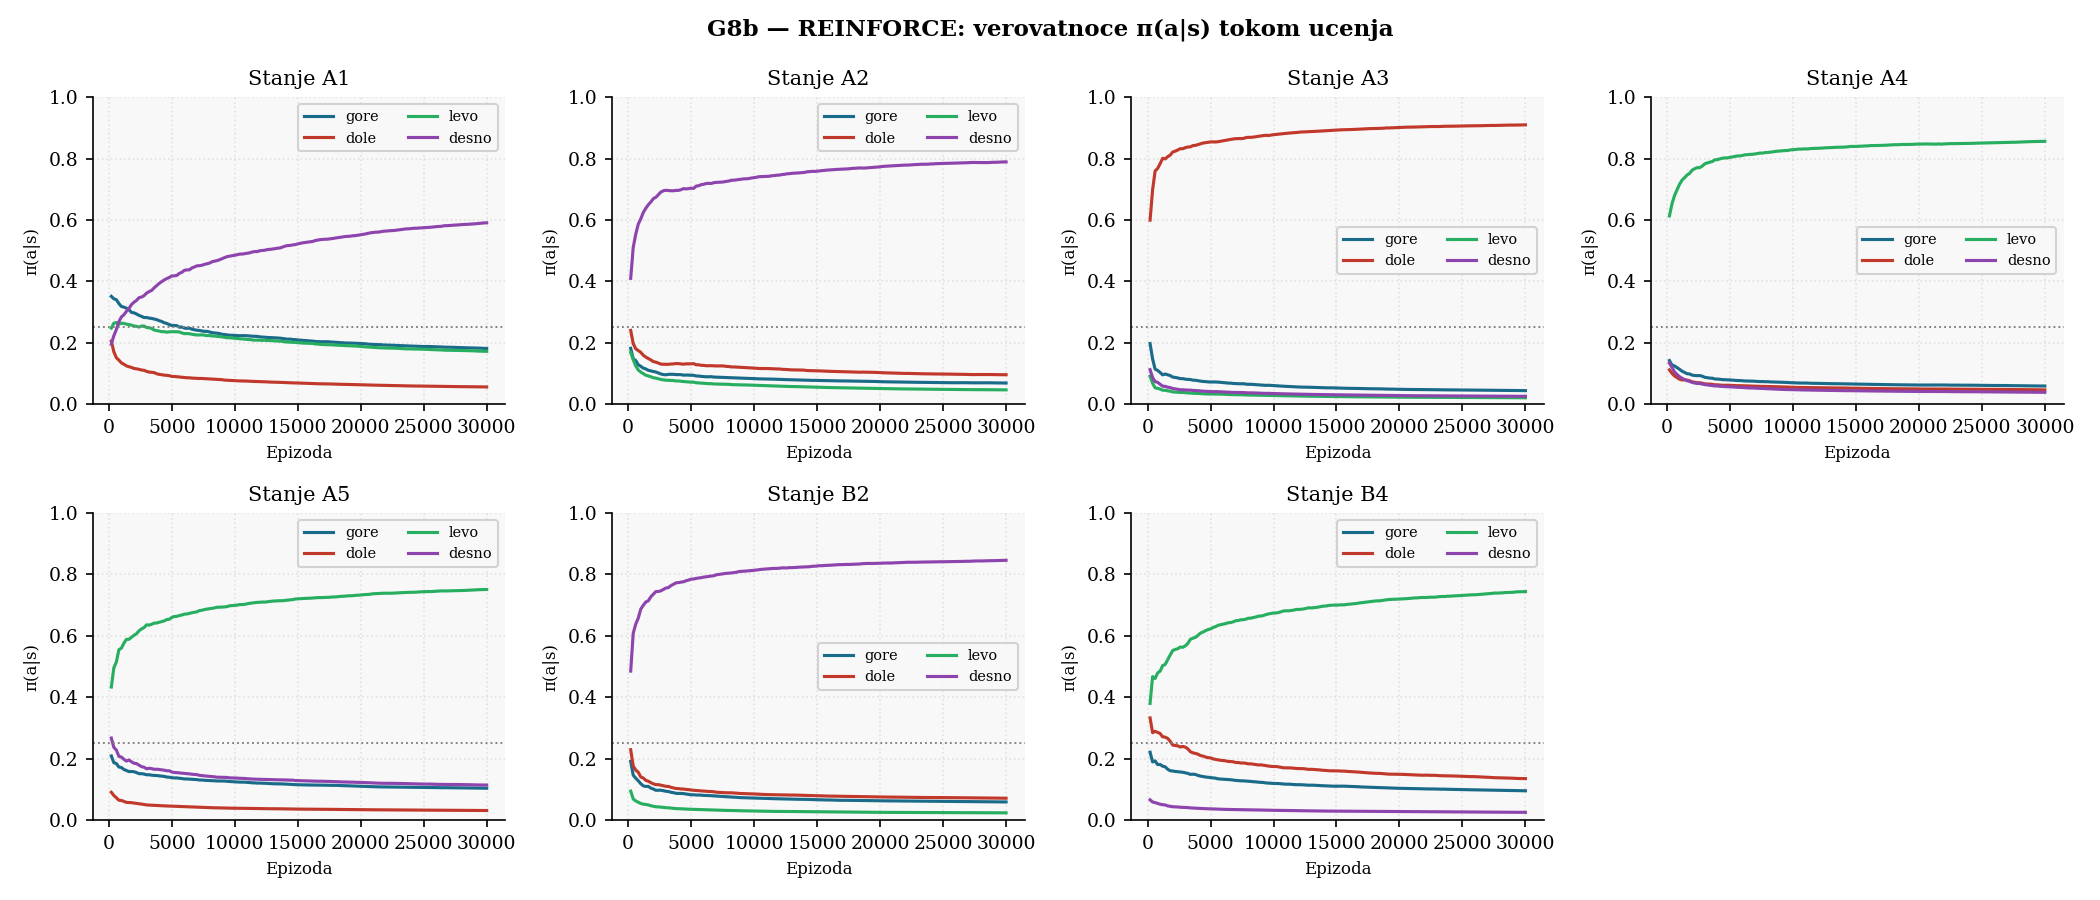
\includegraphics[width=\textwidth]{G8b_RF_pi.png}
  \caption{Verovatnoće akcija $\pi_\theta(a \mid s)$ tokom učenja.
           Isprekidana siva linija označava uniformnu politiku ($1/4 = 0{,}25$).
           Politika postaje sve determinističkija: u finalnoj iteraciji, optimalna akcija
           u stanju $A_3$ ima verovatnoću $91{,}9\%$;
           u ostalim stanjima optimalne akcije imaju verovatnoće $74$--$82\%$.
           Za razliku od Q-učenja koje daje determinističku greedy politiku,
           REINFORCE zadržava stohastičku politiku jer softmaks nikad ne dostiže 1
           ni za jednu akciju.}
  \label{fig:g8b}
\end{figure}

\subsection{Poređenje stopa učenja}

\begin{figure}[H]
  \centering
  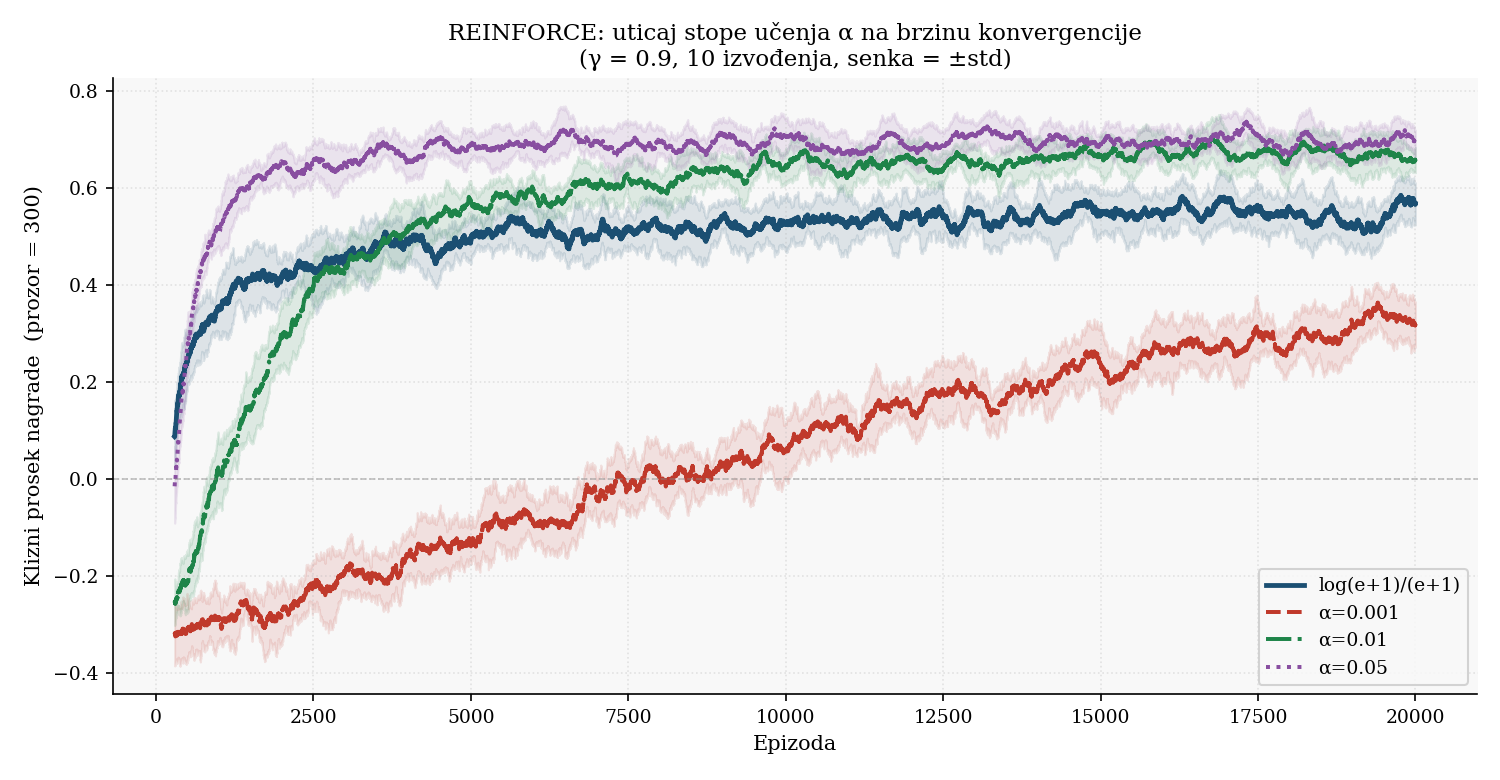
\includegraphics[width=0.90\textwidth]{G9_RF_alpha_poredjenje.png}
  \caption{REINFORCE: poređenje stopa učenja ($\gamma = 0{,}9$, 10 nezavisnih izvođenja,
           20\,000 epizoda, klizni prosek prozorom 300).
           Premala konstanta $\alpha = 0{,}001$ uči previše sporo.
           Vrednost $\alpha = 0{,}01$ postiže dobar napredak ali ne dostiže nivo
           promenljive stope.
           Preveliko $\alpha = 0{,}05$ izaziva nestabilnost (velike oscilacije kliznog proseka)
           jer su moduli return-to-go $|v_\tau|$ znatno veći od 1,
           pa ažuriranja previše pomeraju logite i destabilizuju politiku.
           Promenljiva $\alpha_e = \ln(e+1)/(e+1)$ postiže stabilan, monoton uzlazni trend.}
  \label{fig:g9}
\end{figure}

Napomena: REINFORCE tipično zahteva \emph{manje} stope učenja od Q-učenja jer su
return-to-go vrednosti $v_\tau$ po modulu znatno veće od TD greške $\delta$
(cela suma nagrada vs.\ jedna korekcija).

\subsection{Naučena politika}

\begin{figure}[H]
  \centering
  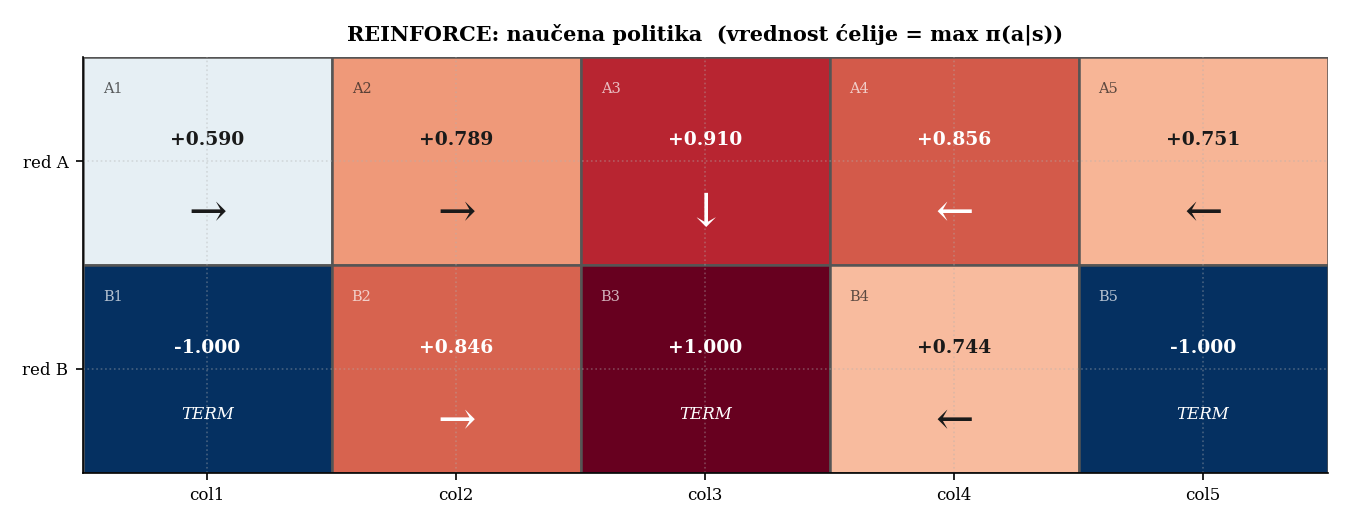
\includegraphics[width=0.85\textwidth]{G10_RF_politika.png}
  \caption{Naučena politika REINFORCE algoritma ($\gamma = 0{,}9$, 30\,000 epizoda).
           Strelice prikazuju $\arg\max_a \pi_\theta(a \mid s)$;
           vrednost u ćeliji je $\max_a \pi_\theta(a \mid s)$
           (mera determinizovanosti, opseg $[0{,}25, 1{,}00]$).
           Politika se u potpunosti poklapa sa $\pi^*$ iz DP etalona:
           svih \textbf{7/7 stanja} ima ispravnu optimalnu akciju.
           Stanje $A_3$ ima najveću sigurnost ($91{,}9\%$);
           ugaona stanja $A_1$ i $A_5$ imaju nešto manje sigurne akcije
           jer su retko posećena tokom učenja.}
  \label{fig:g10}
\end{figure}


% =============================================================================
\section{Sumarno poređenje}
% =============================================================================

\begin{figure}[H]
  \centering
  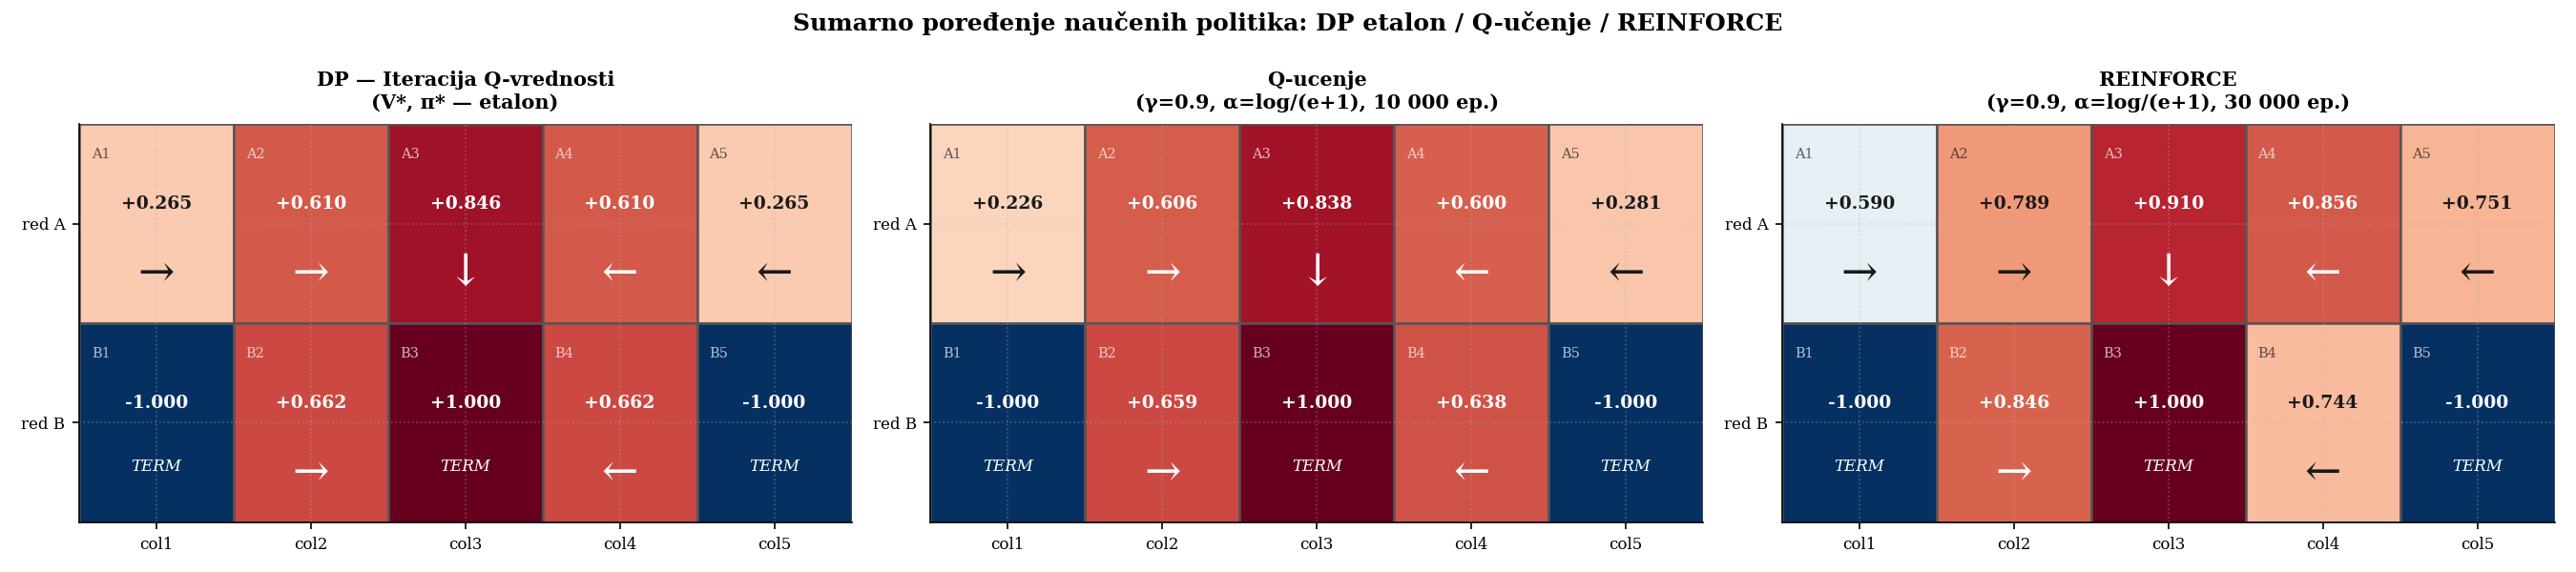
\includegraphics[width=\textwidth]{G11_sumarno.png}
  \caption{Sumarno poređenje tri metode ($\gamma = 0{,}9$):
           iteracija Q-vrednosti (levo, etalon),
           Q-učenje (sredina, 10\,000 epizoda),
           REINFORCE (desno, 30\,000 epizoda).
           Vrednosti u ćelijama: za DP i Q-učenje su $V^*(s)$ i $V_t(s)$ respektivno;
           za REINFORCE je $\max_a \pi_\theta(a \mid s)$.
           Sve tri metode pronalaze istu optimalnu politiku (7/7 poklapanja);
           razlika u numeričkim vrednostima ($V_t$ vs $V^*$) u Q-učenju
           je rezidualni šum posle 10\,000 epizoda, ne sistemska greška.}
  \label{fig:g11}
\end{figure}

\begin{table}[H]
  \centering
  \caption{Poređenje tri metode učenja.}
  \begin{tabular}{llll}
    \toprule
    Osobina & \textbf{Iteracija Q-vred.} & \textbf{Q-učenje} & \textbf{REINFORCE} \\
    \midrule
    Pristup        & Model-based (DP) & Model-free (TD) & Model-free (PG) \\
    Šta uči        & $Q^*(s,a)$       & $Q^*(s,a)$      & $\pi_\theta(a \mid s)$ \\
    Parametri      & n.p.             & $Q$-tabela (28) & $\theta$-tabela (28) \\
    Pristrasnost   & Nema (egzaktno)  & Ima (bootstrap) & Nema (MC) \\
    Varijansa      & n.p.             & Niska           & Visoka \\
    Potrebno       & 53 DP iteracija  & 10\,000 ep.     & 30\,000 ep. \\
    Politika       & Deterministička  & Deterministička & Stohastička \\
    Poklapanje s $\pi^*$ & 7/7       & 7/7             & 7/7 \\
    \bottomrule
  \end{tabular}
  \label{tab:summary}
\end{table}

Sve tri metode konvergiraju ka istoj optimalnoj politici:
u stanjima $A_1$, $A_2$, $B_2$ optimalna akcija je \emph{desno};
u $A_4$, $A_5$, $B_4$ je \emph{levo};
a u $A_3$ je \emph{dole} (direktno ka $B_3$).
Ova simetrična politika odražava simetričnu strukturu okruženja i nagrade.

Ključne razlike između metoda:
\begin{itemize}
  \item \textbf{Iteracija Q-vrednosti} daje egzaktno rešenje u samo 53 iteracije,
    ali zahteva poznat model prelaza (u praksi najčešće nedostupno).
  \item \textbf{Q-učenje} konvergira brže od REINFORCE (manje epizoda, manja varijansa)
    zahvaljujući bootstrappingu, ali uvodi pristrasnost.
    Konačna politika je deterministička greedy politika.
  \item \textbf{REINFORCE} je teorijski nepristrasan (MC procena gradijenta),
    ali mu je potrebno trostruko više epizoda zbog visoke varijanse.
    Daje stohastičku politiku koja se asimptotski približava optimalnoj determinističkoj.
    Varijansa bi se mogla smanjiti dodavanjem \emph{bazne linije} (b),
    što je osnova akter-kritičar arhitektura:
    $\nabla J \propto (v_\tau - b) \cdot \nabla\ln\pi$, ali to nije traženo u ovom zadatku.
\end{itemize}

\end{document}
